\documentclass{article}
\usepackage{amsmath}
\usepackage{amssymb}
\usepackage{bbm}
\usepackage{geometry}

\begin{document}

\section*{Proof of the Campbell Formula}

Let \( C(A \times \Gamma) \) denote the non-reduced Campbell measure for a point process \( X \), where \( A \subset \mathbb{R}^d \) is a set in space, and \( \Gamma \in \mathcal{N}_{\text{lf}} \) is a subset of the possible marks of the points in the process. The non-reduced Campbell measure is given by:

\[
C(A \times \Gamma) = \mathbb{E}\left[ \int_A \mathbbm{1}\{ N(x) \in \Gamma \} \, dN(x) \right],
\]
where \( N(x) \) represents the point process at location \( x \), and \( \mathbbm{1}\{ N(x) \in \Gamma \} \) is the indicator function which is 1 if \( N(x) \in \Gamma \) and 0 otherwise.

\noindent Now, define the function \( f(x, N) = \mathbbm{1}\{ x \in A, N \in \Gamma \} \). We aim to compute the integral of this function over \( \mathbb{R}^d \times \mathcal{N} \) with respect to the Campbell measure.

\[
\int_{\mathbb{R}^d \times \mathcal{N}} f(x, N) \, dC(x \times N) = \int_{\mathbb{R}^d \times \mathcal{N}} \mathbbm{1}\{ x \in A, N \in \Gamma \} \, dC(x \times N).
\]

By the definition of the non-reduced Campbell measure, we have:

\[
\int_{\mathbb{R}^d \times \mathcal{N}} 1\{ x \in A, N \in \Gamma \} \, dC(x \times N) = \int_A P_x(\Gamma) \, dM(x),
\]
where \( P_x(\Gamma) \) is the Palm distribution, which gives the probability that a point at location \( x \) has a mark in \( \Gamma \), and \( M(x) \) is the mean measure (or intensity measure) of the point process. 

Thus, the Campbell formula is:

\[
C(A \times \Gamma) = \int_A P_x(\Gamma) \, dM(x).
\]

This formula expresses the expected number of points in \( A \) with marks in \( \Gamma \), and is derived from the non-reduced Campbell measure and the Palm distribution.


\section*{Palm Probability and Nearest Neighbour Distance in a Poisson Process}

\section*{Theorem}
Let \( X \) be a Poisson point process with intensity measure \( M \), and let \( B_x(r) \) denote the ball of radius \( r \) centered at a fixed point \( x \in \mathbb{R}^d \). Then, the probability that the distance from \( x \) to its nearest neighbour is greater than \( r \) is given by:
\[
\mathbb{P}_x(R^*(x, X) > r) = \exp\left(-M(B_x(r))\right),
\]
where \( M(B_x(r)) \) is the intensity measure of the ball \( B_x(r) \).

\section*{Proof}
We aim to compute the probability that the distance from \( x \) to its nearest neighbour in the Poisson point process \( X \) is greater than \( r \), i.e., 
\[
\mathbb{P}_x(R^*(x, X) > r) = \mathbb{P}_x\left(X \cap (B_x(r) \setminus \{x\}) = \emptyset\right).
\]
This is the probability that there are no points in the ball \( B_x(r) \) (except for the point \( x \)).

\subsection*{Step 1: Conditional Distribution under the Palm Measure}
Under the Palm distribution \( \mathbb{P}_x \), we treat \( x \) as a fixed point in the Poisson point process, and we look at the distribution of the remaining points in \( X \), conditioned on the presence of \( x \).
Since the Poisson point process has independent increments, the remaining points (other than \( x \)) follow a Poisson point process with intensity measure \( M \) in the region \( \mathbb{R}^d \setminus \{x\} \).

\subsection*{Step 2: Distribution of Points in \( B_x(r) \)}
The number of points in the ball \( B_x(r) \), other than \( x \), is a Poisson random variable with mean \( M(B_x(r)) \), i.e.,
\[
\text{Poisson}(M(B_x(r))).
\]
Therefore, the probability that there are no points in \( B_x(r) \) other than \( x \) is:
\[
\mathbb{P}_x\left( X \cap (B_x(r) \setminus \{x\}) = \emptyset \right) = \exp\left(-M(B_x(r))\right).
\]

\subsection*{Step 3: Conclusion}
Thus, the probability that the distance from \( x \) to its nearest neighbour is greater than \( r \) is given by:
\[
\mathbb{P}_x(R^*(x, X) > r) = \exp\left(-M(B_x(r))\right),
\]
which completes the proof.
\begin{figure}[h!]
    \centering
    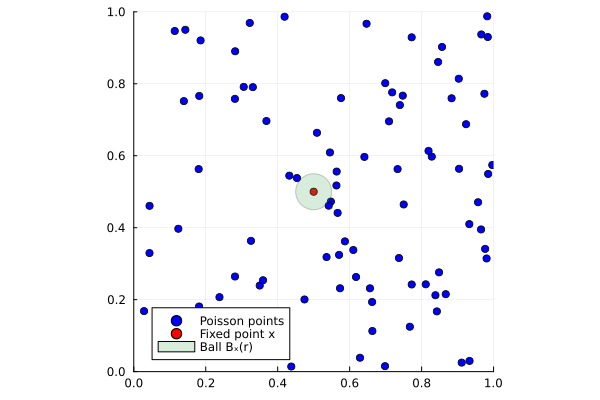
\includegraphics[width=\textwidth]{conditioned_realisation.pdf}
    \caption{Ex.}
\end{figure}


\end{document}

